\section{Mobile platforms and the market}

The demand for applications to be portable on mobile phones and tablets has become a fashion as well as accessibility on the go. In the current market Cryptic crosswords are available in a variety of newspapers, magazines and online websites. These are everyday media in which a person can access their favourite Cryptic Crosswords and participate in. With the expansion of mobile phone and tablet applications research has shown that a unique Cryptic Crossword solver has not been incorporated in any of the mobile operating systems. There are applications, which can be downloaded, that are pre-solved crosswords but there is no real solver, which solves Cryptic Crosswords in real time. In fact research has shown that there is only a very small handful of Cryptic Crossword applications across all mobile operating systems.

\subsection{Mobile Operating Systems}

The Oxford English dictionary states an ``Operating System'' as `the low-level software that supports a computer’s basic functions, such as scheduling tasks and controlling peripherals' \citep{oxford_dictionary11}.

A mobile operating system has the same definition but supports the basic functions for handheld devices such as mobile phones and tablets. In the current market the term mobile operating system is associated with smartphones rather than mobile phones due to the powerful processors, which are embedded in the mobile phone devices. 

The official first mobile operating system for smartphones was by IBM introduced in 2000 as the `Simon' but it was Ericson who created the first all in one smartphone with the Symbian OS, which incorporated a keyboard hence, the term smartphone was introduced. This ran on various mobile phones by companies such as Ericcson, Samsung but predominantly on smartphones by Nokia. This created a path for a market, which was to be dominated by others in the coming future \citep{smartphone11}.

By 2007 from the back of a successful campaign selling music devices known as the iPod, Apple introduced the Apple IPhone which came with their fist mobile operating system the IOS which was a full operating system used from the Mac OS X 10 \citep{macworld07}.

By July 2008 Apple released IOS 2.0 and with this came the app store. This was a revolution to the mobile market allowing a platform for third party developers to sell and market their own applications for the mobile operating system. On the 7th January 2013 Apple announced that they have had more than 40 Billion downloads of apps through their app store \citep{40billion12}.

In September 2008 Google released their own version of a mobile operating system ‘Android’ which had its similarities of marketing with its very own app store known as the android market which since has been rebranded to the Google play store. 

In April 2009 Blackberry also launched it’s own application store called the Blackberry World, which works with their mobile operating system the Blackberry 10 \citep{bbworld09}.

Finally windows released their version of an app store for distribution of applications on October 26th 2012 \citep{windows8}.

Although there are now several platforms that run on a mobile device, Android and iOS combine for 91.1\% of the Worldwide Smartphone OS Market \citep{idc13}.

This shows that although blackberry has been in the market since 2009 there isn’t much of a rise to interests in their apps and while Windows is fairly new it has a lot of ground to cover to catch up with their main competitors.

For the purpose of this project it is pretty clear to what is demanded from consumers in the real world with Apple and Google being the two main competitors for mobile applications. In order to decide on what platform the project will be suitable for to design, maintain and deploy a good working product below is the following page contains a table which covers some of the reasons which could be possible to allow the team members to come to a decision to what pathway the project will be going in.

\newpage
\begin{landscape}
\begin{table}
    \begin{tabular}{|l|l|l|l|l|l|l|}
    \hline
                      Platform & Programming Language & Open Source & Open API/SDK & License     & Underlying OS & Development Environment \\ \hline
    Android                    & Java                 & Yes         & Yes          & Apache      & Linux         & Eclipse                 \\ \hline
    IOS                        & Objective C          & N/A         & Yes          & Proprietary & Darwin        & XCode                   \\ \hline
    Blackberry                 & Java, C++            & N/A         & Yes          & Proprietary & Blackberry OS & Eclipse                 \\ \hline
    Windows                    & C, C++, C\#           & N/A         & Yes          & Microsoft   & Windows       & Visual Studio           \\ \hline
    \end{tabular}
    \caption {A comparison of mobile platforms}
\end{table}


\begin{table}
    \begin{tabular}{|l|l|l|l|l|l|l|}
    \hline
    Platform   & Latest Version    & Debugging & Hardware/ Software Requirements & Emulator & Submission to app store & Development Cost                            \\ \hline
    Android    & 4.3 Jelly   Bean  & Yes       & Windows   / Mac                 & Yes      & Unlimited               & \$25 One   Off cost                          \\ \hline
    IOS        & IOS 7             & Yes       & Intel   Based Mac               & Yes      & Unlimited               & \pounds60   Yearly / \$99                          \\ \hline
    Blackberry & Blackberry   10   & Yes       & Windows/Mac                     & Yes      & 100 Per   Year          & \$100   One off cost                         \\ \hline
    Windows    & Windows   Phone 8 & Yes       & Windows                         & Yes      & Unlimited               & \$19   Yearly / Free for Dreamspark Students \\ \hline
    \end{tabular}
    \caption {A further comparison of mobile platforms}
\end{table}

\end{landscape}

Although these are the four main types of platforms available in the market for mobile development there is a growing amount of organisations, which are developing tools to allow developers to create cross platform application with ease. Two of these are Appcelerator and Adobe AIR.

\begin{table}
    \begin{tabular}{|l|l|l|l|l|l|l|}
    \hline
    Platform     & Programming   Language              & Open Source & Open API/SDK & License     & Underlying OS & Development   Environment          \\ \hline
    Appcelerator & JavaScript                          & Yes         & Yes          & Apache 2.0  & Linux         & Eclipse Based IDE/ Titanium Studio \\ \hline
    Adobe AIR    & ActionScript, HTML, CSS, JavaScript & No          & Yes          & Proprietary & Darwin        & Adobe AIR                          \\ \hline
    \end{tabular}
     \caption {A comparison of cross platform development tools}
\end{table}

\subsection{Appcelerator}

Appcelerator is a platform created by Appcelerator Inc to allow developers to create cross platform native applications for Android and IOS. They later introduced compatibility for Blackberry 10 and are in the process of developing for Windows Phone. The main development environment used to create applications is an Eclipse based IDE known as Titanium Studio. Developers can create great looking native apps using JavaScript. The use and license of Appcelerator falls under Apache 2.0.

\subsection{Adobe AIR}

Adobe Integrated Runtime (Adobe AIR) uses adobe tools such as flash to allow developers to create platform independent web apps. Unlike Appcelerator this means that applications created can only be web based and not native. For this reason a lot of developers avoid using Adobe AIR. It supports all the major vendors for mobile applications but apps created in Adobe AIR are a lot slower.

\subsection{Native Apps}

A native app is a platform independent application designed to work with a particular mobile OS. The app is installed on the device whether it’s a smartphone or a tablet.

Advantages

\begin{itemize}
    \item Faster at accessing device features such as camera and accelerometer
    \item Easy to find in app stores such as Google Play and Apple app store
    \item Secure as they go through an approval phase from vendors 
\end{itemize}


Disadvantages

\begin{itemize}
    \item Expensive to develop 
    \item Expensive to maintain 
    \item Approval process can take from days to months
    \item Support of the app can be hard to maintain due to different people using different versions of operating system installed.
\end{itemize}

\subsection{Web Apps}

A web application is really a website designed to look and feel like an app. This is wrapped by the web browser, which means an Internet connection is required to use the app. Google Chrome and Safari are examples of Web apps. 

Advantages

\begin{itemize}
    \item Easy to maintain 
    \item Can be compatible with any device 
    \item Approval is not required
    \item Easy to maintain and update without affecting the user to update the software 
\end{itemize}

Disadvantages
\begin{itemize}
    \item Limited to what can be accessed on the devices 
    \item Hard to provide support over various Web browsers
    \item Not easy to find and promote, users will have to browse websites 
    \item Can be insecure due to the application being web based 
\end{itemize}

There are various platforms available for mobile devices. The most popular platforms are the as previously mentioned. Although they are in contest the use and popularity of platforms vary from region to region. An article published by \citet{wpcentral13} states that windows phone is the most popular platform in Latin America. Although the platform was produced later than the other platforms this has become popular due to the lower prices of devices. Devices such as the IPhone and the IPad are a lot dearer and can cost a user a couple of hundred pounds. In September Forbes reported that the most popular platform on mobile devices is Android. 

\newpage
\begin{figure}[!ht]
    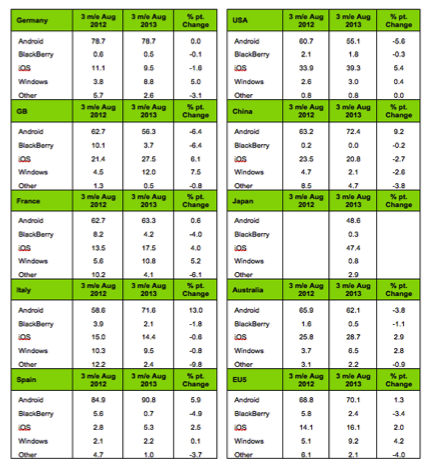
\includegraphics[width=\linewidth]{research/mobile_platforms/forbeslist13.png}
    \caption{Mobile phone market share September 2013}
\end{figure}

\begin{flushright}
    \citep{forbes13}
\end{flushright}

\subsection{Currently available Cryptic Crossword apps}

After performing various research on the apple app store, the Google play store and blackberry world, it was discovered that there is not many Cryptic Crosswords available to download. There were two, which could be clearly defined as Cryptic Crossword applications, and these have been analysed in the following sections.

\subsection{Puzzler Super Cryptic Crosswords}

Platform: Apple iOS \\
Price: \pounds3.99 \\
Compatibility: iOS 4.3 or Later \\
Website: https://itunes.apple.com/gb/app/puzzler-super-cryptic-crosswords/id616060420?mt=8

\begin{figure}[!ht]
    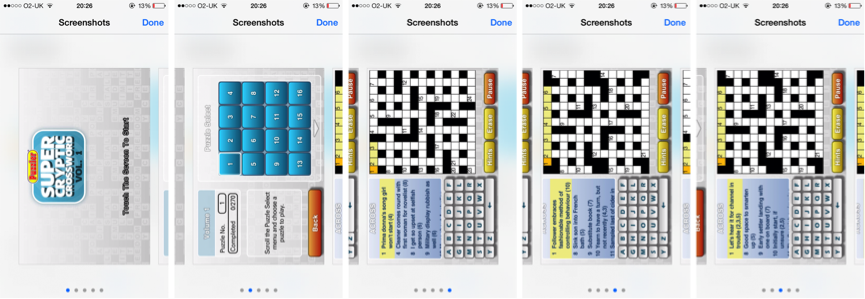
\includegraphics[width=\linewidth]{research/mobile_platforms/pscs.png}
    \caption{Screenshots of Puzzler Super Cryptic Crosswords on IPhone}
\end{figure}

This application contains 270 pre built crosswords. The interface is really easy to use and it clearly shows what has been completed and what needs to be completed. What’s nice about this application is that the crosswords are in various levels and as you complete one crossword you can move on to the next. What was noticed is that the application already stores the answers and also the application allows hints, which makes it a little easier to use. The other noticeable thing about this application is that it didn’t fully use the native features of the mobile phone. Like the keyboard is a custom keyboard. 


\subsection{Cryptic Crossword}

Platform: Apple iOS, Android\\
Price: Free with 2 puzzles on Apple devices- In app purchase avalable - \pounds1.99 on Android Devices\\
Compatibility: iOS 6.0 or Later\\
Website: https://itunes.apple.com/gb/app/cryptic-crossword/id661608021?mt=8


\begin{figure}[!ht]
    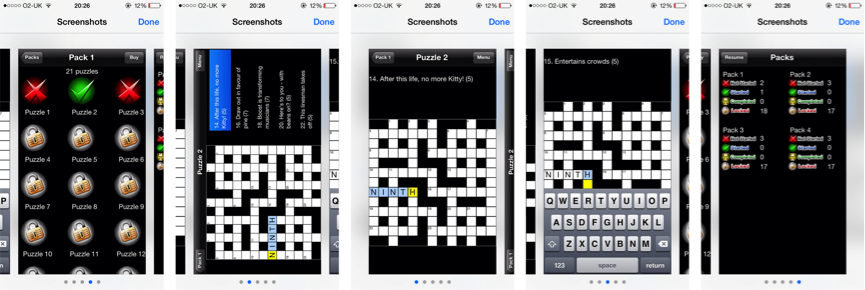
\includegraphics[width=\linewidth]{research/mobile_platforms/cc.png}
    \caption{Screenshots of Cryptic Crossword on IPhone}
\end{figure}

The Cryptic Crosswords app comes with 4 different packages and a total of 81 puzzles. Each pack can be bought for \pounds0.69 or all 4 for a discounted price of \pounds1.99. Each package contains various cryptic crossword puzzles. After having a play around with this application at first point of contact it is noticed that look and feel of the application is not that great. The use of colours and the layout styles of the application can be better. The app consists of 81 puzzles, which can be played only after each crossword has been completed. Some of the features of the app are:

\begin{itemize}
    \item Checking answears
    \item Revealing a letter, a word or the whole puzzle
    \item Clearing the puzzle
    \item Moving the character bar to next box
    \item Greying out completed clues
\end{itemize}

These are some of the features the application uses but there are plenty more. 

